\documentclass[letterpaper,11pt]{ctexart}
% Original Chinese resume retained as the source-language reference.

% ==================== Packages ====================
\usepackage[empty]{fullpage}
\usepackage{titlesec}
\usepackage[dvipsnames, svgnames, x11names]{xcolor}
\usepackage{enumitem}
\usepackage{hyperref}
\usepackage{fancyhdr}
\usepackage{tabularx}
\usepackage{fontawesome5}
\usepackage{graphicx}
\usepackage{array}
\usepackage{geometry}
\usepackage{needspace}

% ==================== Page Settings ====================
\geometry{
    left=0.45in,
    right=0.45in,
    top=0.38in,
    bottom=0.42in,
    nohead
}

\pagestyle{fancy}
\fancyhf{}
\fancyfoot{}
\renewcommand{\headrulewidth}{0pt}
\renewcommand{\footrulewidth}{0pt}
\setlength{\footskip}{4.1pt}

\raggedbottom
\raggedright
\setlength{\tabcolsep}{0in}
\urlstyle{same}

% ==================== Colors ====================
\definecolor{link}{RGB}{34,78,160}
\definecolor{textgray}{RGB}{70,70,70}
\definecolor{lightgray}{RGB}{220,220,220}

\hypersetup{
    colorlinks=true,
    urlcolor=link,
    linkcolor=link,
    pdftitle={邢梓韬个人简历},
    pdfauthor={邢梓韬}
}

% ==================== List Settings ====================
\setlist[itemize]{
    topsep=0.15em,
    itemsep=0.05em,
    parsep=0em,
    leftmargin=1.4pc
}

\renewcommand\labelitemi{\raisebox{0.2ex}{\tiny$\bullet$}}

% ==================== Custom Commands ====================
\newcommand{\SectionFont}{\fontsize{15.2pt}{17pt}\selectfont}

\titleformat{\section}{
    \vspace{-2pt}
    \color{link}
    \scshape\raggedright\SectionFont\bfseries
}{}{0em}{}[
    \vspace{-3pt}
    \color{link}\titlerule
    \vspace{-5pt}
]

\newcommand{\resumeSubheading}[4]{
    \vspace{3pt}
    \noindent
    \begin{tabular*}{\textwidth}{l@{\extracolsep{\fill}}r}
        \textbf{#1} & \textbf{#2} \\
        \textit{\textcolor{textgray}{#3}} & \textcolor{textgray}{#4} \\
    \end{tabular*}
    \vspace{-3pt}
}

\newcommand{\resumeProject}[4]{
    \vspace{3pt}
    \noindent
    \begin{tabular*}{\textwidth}{l@{\extracolsep{\fill}}r}
        \textbf{#1} & \textbf{#2} \\
        \textit{\textcolor{textgray}{#3}} & \textcolor{textgray}{#4} \\
    \end{tabular*}
    \vspace{-3pt}
}

\newcommand{\contactItem}[2]{
    \makebox[1.25em][c]{\textcolor{link}{#1}} \ #2
}

\newcommand{\skillItem}[2]{
    \noindent
    \begin{tabular*}{\textwidth}{@{}p{2.4cm}@{\extracolsep{\fill}}p{14.3cm}@{}}
        \textbf{#1} & #2
    \end{tabular*}
    \vspace{1pt}
}

% ==================== Document ====================
\begin{document}

% ==================== Header ====================
\vspace{2pt}

\begin{minipage}[c]{0.22\textwidth}
    \centering
    {\setlength{\fboxsep}{2pt}
    \fcolorbox{lightgray}{white}{
        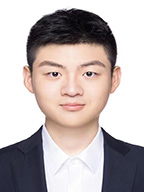
\includegraphics[width=3.0cm, height=3.6cm, keepaspectratio]{照片.jpg}
    }}
\end{minipage}
\hfill
\begin{minipage}[c]{0.74\textwidth}
    \raggedleft

    {\Huge \textbf{\textcolor{link}{邢梓韬}}} \\[5pt]

    {\small
    \contactItem{\faIcon{map-marker-alt}}{厦门大学，福建省厦门市，361005} \\[3pt]
    \contactItem{\faIcon{phone}}{(+86) 18121271166} \\[3pt]
    \contactItem{\faIcon{envelope}}{\href{mailto:vincentxingzitao@gmail.com}{vincentxingzitao@gmail.com}} \\[3pt]
    \contactItem{\faIcon{github}}{\href{https://github.com/VincentXing23}{github.com/VincentXing23}} \\[3pt]
    \contactItem{\faIcon{globe}}{\href{https://zitao-xing-homepage.vercel.app}{zitao-xing-homepage.vercel.app}}
    }
\end{minipage}

\vspace{7pt}

% ==================== Education ====================
\section{教育经历}

\resumeSubheading
{厦门大学}
{中国厦门}
{应用数学--运筹学学术硕士--保研}
{2026年9月入学}

\resumeSubheading
{厦门大学}
{中国厦门}
{数学专业本科生}
{2022年9月 -- 2026年6月}

\vspace{2pt}

\resumeSubheading
{加州大学圣地亚哥分校}
{美国加利福尼亚州圣地亚哥}
{UPS 项目}
{2024年9月 -- 2024年12月}

\vspace{1pt}
\noindent
\textbf{GPA}: 3.4/4.0
\quad
\textbf{平均分}: 85/100
\quad
\textbf{年级排名}: 16/49

% ==================== Internships ====================
\section{实习经历}

\resumeProject
{上海人工智能研究院}
{上海}
{算法实习生}
{2026年8月 -- 至今}
\begin{itemize}
  \item 围绕 AI for Science 方向开展科研复现，梳理研究问题、方法流程、实验配置与评价方式。
  \item 将复现结果与论文报告或基线结果进行对照，记录实现选择、实验现象与尚待分析的差异。
\end{itemize}

\resumeProject
{\href{https://github.com/easyhang/evo_wiki}{上海市大数据股份有限公司（Evo Wiki）}}
{上海}
{人工智能开发实习生}
{2026年7月 -- 2026年8月}
\begin{itemize}
  \item 参与 Evo Wiki 的开发与迭代，围绕 AI 原生 Wiki 与 LightRAG 工作流改进知识组织、检索和交付能力。
  \item 探索法律语料的知识图谱抽取与检索增强生成流程，关注实体关系建模、检索质量和证据可追溯性。
\end{itemize}

\resumeProject
{嘉实基金管理有限公司}
{上海}
{上海区域实习生}
{2025年1月 -- 2025年3月}
\begin{itemize}
  \item 参与上海区域业务支持工作，协助完成基金产品、市场动态与客户服务材料的整理，提高对资产管理行业、基金产品体系与机构业务流程的理解。
  \item 使用 Excel、PPT 等工具完成市场信息、产品资料与同业数据的基础汇总、清洗、排版和展示材料制作。
  \item 支持区域团队日常运营与活动准备，包括会议材料整理、客户沟通资料归档、路演及培训材料辅助制作等工作。
  \item 在实习过程中提升金融行业信息整理、数据处理、材料表达与跨团队沟通能力，为后续 AI 与金融数据分析结合打下基础。
\end{itemize}

% ==================== Research and Projects ====================
\Needspace{8\baselineskip}
\section{科研与项目经历}

\resumeProject
{\href{https://github.com/Romanrose/shangtu-notebook}{上海图书馆开放数据竞赛：时空探索手札}}
{上海}
{项目成员}
{2026年8月}
\begin{itemize}
  \item 参与研发面向平板触控场景的 PWA，支持用户在数字纸页上手写人物、地点、经历与作品等内容。
  \item 参与打通手写转写、受控知识图谱检索、来源证据核验与可追溯旁批等流程。
\end{itemize}

\resumeProject
{\href{https://github.com/VincentXing23/Graphrag-for-Network/tree/main}{基于 BGP 网络数字孪生的 GraphRAG MVP}}
{个人项目}
{项目开发者}
{2026年7月 -- 至今}
\begin{itemize}
  \item 构建基于 BGP 控制面状态的网络数字孪生 MVP，将 FRR 风格路由状态转换为版本化网络快照，实现确定性的路径查询与变更前后影响分析。
  \item 实现样例、FRR/containerlab 实验网络与合成规模化三种运行模式；规模场景覆盖 4 个区域、100 台设备与每快照 12,000 条路由记录，并以新鲜度标记处理局部采集失败。
  \item 集成 Neo4j 图存储、Qdrant/向量检索回退与兼容 OpenAI 或本地模型的 GraphRAG 层，为网络路径与变更结果提供带证据的解释。
  \item 通过 Python CLI、FastAPI、Docker Compose 与 Cytoscape 工作台提供系统能力，展示网络拓扑、路径变化、采集状态和检索证据。
\end{itemize}

\resumeProject
{香港中文大学（深圳）AISE 人工智能+理工科夏令营}
{广东深圳}
{营员}
{2025年7月 -- 2025年8月}
\begin{itemize}
  \item 系统学习深度学习与 AI for Science 相关内容，掌握神经网络结构、反向传播、梯度下降优化、损失函数设计、模型训练与评估等核心流程。
  \item 参与完成神经网络训练项目，负责数据预处理、模型结构搭建、训练调参与实验结果分析，形成从问题建模、模型训练到结果展示的完整实践流程。
  \item 学习 GPU 并行计算与 CUDA 编程基础，理解线程组织、内存管理、并行加速与科学计算中的 GPU 计算思想，提升深度学习与高性能计算结合的实践能力。
  \item 使用 Python 及深度学习框架完成模型训练，结合数学优化背景分析学习率、训练轮数、网络结构等超参数对模型收敛与泛化表现的影响。
\end{itemize}

\vspace{2pt}

\resumeProject
{科研攀登计划（国家级）——泛函分析课程 GraphRAG：建设与可行性验证}
{福建厦门}
{项目负责人}
{2025年5月 -- 2026年5月}
\begin{itemize}
  \item 主持国家级科研训练项目，面向泛函分析课程构建知识图谱增强检索系统，负责项目统筹、技术方案整合、系统验证与成果展示材料整理。
  \item 完成课程资源结构化建模，将章节、知识点、定理、例题和问题抽象为课程对象，并设计对应的图谱关系。
  \item 构建包含 95 个课程对象与 216 条图谱关系的课程知识图谱，覆盖章节、知识点、定理、例题和问题等对象类型，支撑课程知识的层级化与关联化组织。
  \item 基于 Neo4j、Qdrant、BAAI/bge-m3、BAAI/bge-reranker-v2-m3 与 Flask 搭建本地 GraphRAG demo，实现自然语言检索、向量召回、reranker 重排、图谱上下文扩展与流程可视化。
  \item 完成样例查询与系统验证，跑通“自然语言问题 $\rightarrow$ 课程对象召回 $\rightarrow$ 结果重排 $\rightarrow$ 图谱上下文扩展 $\rightarrow$ 证据链展示”的原型链路，并探索接入阿里云智能体与智慧树课程平台的应用场景。
\end{itemize}

\vspace{2pt}

\Needspace{14\baselineskip}
\resumeProject
{大学生创新创业项目（省级）——偏微分方程的新型数值方法研究}
{福建厦门}
{项目成员}
{2025年4月 -- 2026年4月}
\begin{itemize}
  \item 围绕扇形域上 Poisson 方程的数值求解开展研究，重点关注角点奇性与非光滑结构对传统数值逼近方法精度的影响。
  \item 参与设计匹配角点奇异结构的 Müntz 型基函数方法，并与普通代数幂基方法、神经网络辅助 baseline 进行对比，分析不同近似空间对误差表现的影响。
  \item 完成一维奇异函数逼近、扇形域 Poisson 方程单模态与双模态基准问题、奇异指数匹配/不匹配消融实验等数值实验，整理误差数据与可视化结果。
\end{itemize}



\vspace{2pt}
% ==================== Honors ====================

\section{竞赛与荣誉}

\begin{itemize}
    \item \textbf{2023年外研社·国才杯全国英语写作/演讲类竞赛}，省级\textbf{二等奖}
    \begin{itemize}
        \item 系统训练英文写作、逻辑论证与结构化表达能力，具备较好的英文材料阅读、整理与汇报基础。
    \end{itemize}

    \item \textbf{2023年全国大学生数学建模竞赛}，省级\textbf{三等奖}
    \begin{itemize}
        \item 参与数学模型构建、算法设计、数值实验与论文撰写，提升从实际问题中抽象数学模型、开展数据分析与团队协作的能力。
    \end{itemize}

    \item \textbf{爱XIA创：厦门黑客松 AI for Science / Agent 赛道}，\textbf{三等奖}
    \begin{itemize}
    \item 参与 SciVisualizer 科研智能体项目，围绕 AI for Science 场景梳理科研工作流痛点，协助将“自然语言科学意图输入—Agent 解析—算力任务调度—可视化渲染—报告输出”的流程转化为可展示的产品方案。
    \item 重点参与智能体与工作流的设计优化，协助拆解科研任务中的建模、计算提交、结果解析、可视化展示等环节，提升系统在科学计算场景下的自动化程度与用户交互清晰度。
    \item 结合数学与科研训练背景，参与科学问题抽象、应用场景建模和路演材料打磨，突出 Agent 工作流在降低工具链割裂、提升科研效率和支持 AI for Science 应用落地方面的价值。
    \end{itemize}

\end{itemize}



% ==================== Skills ====================
\section{技能与兴趣}

\skillItem{编程语言}{Python，C/C++，MATLAB，CUDA}
\skillItem{工具平台}{Git，VS Code，阿里云}
\skillItem{语言能力}{中文（母语），英文（熟练，雅思 7.0）}
\skillItem{职业兴趣}{应用数学，机器学习，RAG，运筹学，图算法，AI for Science，Agent 开发}
\skillItem{业余爱好}{茶文化，咖啡，羽毛球，长跑}
\end{document}
